\documentclass{article}[10pt]
\usepackage[margin=1in]{geometry}
\pagenumbering{gobble}

\usepackage{times}
\usepackage[usenames,dvipsnames,svgnames,table]{xcolor}
\usepackage{boxedminipage}
\usepackage{xspace}
\usepackage{pifont}
\usepackage{fancyvrb}
\usepackage{wrapfig}
\usepackage{graphicx}
\usepackage{amsmath}
\usepackage{textgreek}

\definecolor{MyDarkBlue}{rgb}{0,0.08,0.45}
\usepackage[pdftex]{hyperref}
\hypersetup{
    colorlinks,%
    citecolor=MyDarkBlue,%
    filecolor=MyDarkBlue,%
    linkcolor=MyDarkBlue,%
    urlcolor=MyDarkBlue
}
\usepackage{fixltx2e}
\usepackage[sort]{cite}

\makeatletter
\newcommand*{\rom}[1]{\expandafter\@slowromancap\romannumeral #1@}
\makeatother

%,xcolor,rotating,graphicx,graphics,url,epsfig,
%amsfonts,algpseudocode,xspace,amsmath,amssymb,fancyvrb,fixltx2e

% Ethan hacks:----------
\setlength{\pdfpagewidth}{8.5truein}
\setlength{\pdfpageheight}{11truein}

%%% format things for making pretty tables using booktabs package
\usepackage{multirow}
\usepackage{booktabs}
\setlength{\heavyrulewidth}{0.10em}
\setlength{\lightrulewidth}{0.05em}
\setlength{\cmidrulewidth}{\lightrulewidth}
\setlength{\cmidrulekern}{0em}%
%
%\let\oldthebibliography=\thebibliography
%\let\endoldthebibliography=\endthebibliography
%\renewenvironment{thebibliography}[1]{%
%\begin{oldthebibliography}{#1}%
%\setlength{\itemsep}{-.3ex}%
%}%
%{%
%\end{oldthebibliography}%
%}

\textfloatsep 10pt plus 3pt minus 2pt   % Space between main text and floats

\newcommand{\squishlist}{
   \begin{list}{$\bullet$}
    { \setlength{\itemsep}{0pt}      \setlength{\parsep}{3pt}
      \setlength{\topsep}{3pt}       \setlength{\partopsep}{0pt}
      \setlength{\leftmargin}{1.5em} \setlength{\labelwidth}{1em}
      \setlength{\labelsep}{0.5em} } }

\newcommand{\squishlisttwo}{
   \begin{list}{$\bullet$}
    { \setlength{\itemsep}{0pt}    \setlength{\parsep}{0pt}
      \setlength{\topsep}{0pt}     \setlength{\partopsep}{0pt}
      \setlength{\leftmargin}{2em} \setlength{\labelwidth}{1.5em}
      \setlength{\labelsep}{0.5em} } }

\newcommand{\squishend}{
    \end{list}  }

%
\def\compactify{\itemsep=2pt \topsep=3pt \partopsep=1pt \parsep=1pt \leftmargin=1.5em}
\let\latexusecounter=\usecounter
\newenvironment{CompactEnumerate}
  {\def\usecounter{\compactify\latexusecounter}
   \begin{enumerate}}
   {\end{enumerate}\let\usecounter=\latexusecounter}
\newenvironment{CompactItemize}
   {\def\usecounter{\compactify\latexusecounter}
   \begin{itemize}}
   {\end{itemize}\let\usecounter=\latexusecounter}

\makeatletter
\renewcommand\section{\@startsection{section}{1}{\z@}%
                                  {-3.5ex \@plus -1ex \@minus -.2ex}%
                                  {2.3ex \@plus.2ex}%
                                  {\normalfont\normalsize\bfseries}}
\makeatother


% Macros:
\newcommand{\projectname}{{STS}}
\newcommand{\projectmeaning}{the SDN Troubleshooting Simulator}

\newcommand{\simulator}{retrospective causal inference}
\newcommand{\Simulator}{Retrospective causal inference}
\newcommand{\SIMULATOR}{RETROSPECTIVE CAUSAL INFERENCE}

\newcommand{\tbd}[1]{{\bf [[TBD: {#1}]]}}
\newcommand{\ie}{{\it i.e.}}
\newcommand{\eg}{{\it e.g.}}
\newcommand{\cf}{{\it cf.}}
\newcommand{\defacto}{{\em de facto}}
\newcommand{\etc}{{\it etc.}}
\newcommand{\viz}{{\it viz.}}
\newcommand{\apriori}{{\it a priori}}
\newcommand{\eat}[1]{}
\newcommand{\primafacie}{{\em prima facie}}

% Notes:
\newcommand{\num}[1]{{\color{red}\bf {#1}}}
%\newcommand{\teemu}[1]{{\color{ForestGreen}\bf TK: {#1}}}
%\newcommand{\andi}[1]{{\color{blue}\bf AW: {#1}}}
%\newcommand{\sam}[1]{{\color{orange}\bf SW: {#1}}}
%\newcommand{\colin}[1]{{\color{red}\bf CS: {#1}}}
%\newcommand{\scott}[1]{{\color{purple}\bf SS: {#1}}}

\newcommand{\teemu}[1]{}
\newcommand{\andi}[1]{}
\newcommand{\sam}[1]{}
\newcommand{\colin}[1]{}
\newcommand{\scott}[1]{}

% Delta-debugging symbols:
\newcommand{\PASS}{\text{\ding{52}}\xspace}
\newcommand{\FAIL}{\text{\ding{56}}\xspace}
\newcommand{\cpass}{{T_{\scriptscriptstyle \PASS}}}
\newcommand{\cfail}{{T_{\scriptscriptstyle \FAIL}}}
\newcommand{\dpass}{{T'_{\scriptscriptstyle \PASS}}}
\newcommand{\dfail}{{T'_{\scriptscriptstyle \FAIL}}}
\newcommand{\done}{{T_{\scriptscriptstyle 1}}}
\newcommand{\dtwo}{{T_{\scriptscriptstyle 2}}}
\newcommand{\test}{\textit{replay}\xspace}
\newcommand{\ddmin}{\textit{ddmin}\xspace}


\sloppy
\begin{document}
    \date{}

\title{{Selective Recall for Troubleshooting SDN Control Software}}

\author{C. Scott$^\dagger$, A. Wundsam$^*$, S.Whitlock$^*$, A. Or$^\dagger$, E. Huang$^\dagger$, K. Zarifis$^\ddagger$, S. Shenker$^\dagger$$^*$,
\and {\begin{tabular}{ccc}$^\dagger${\large\it UC Berkeley} & $^*${\large\it ISCI} & $^\ddagger${\large\it University of Southern California}\end{tabular}}
}
%\and A. Wundsam%\thanks{Big Switch Networks} %
%\and S. Whitlock% \thanks{ICSI}  % 
%\and A. Or% \footnotemark[1] % 
%\and E. Huang%\footnotemark[1] %
%\and K. Zarifis% \thanks{USC} %
%\and S. Shenker% \footnotemark[3]~\footnotemark[1] % 
%\and {\begin{tabular}{ccc}$^\dagger${\large\it UC Berkeley} & $^*${\large\it ISCI} & $^\ddagger${\large\it University of Southern California}\end{tabular}}
%}

\date{}
   \maketitle
   \vspace{-0.3in}
   \thispagestyle{empty}
\label{sec:intro}
The SDN platform's $raison\text{ }d'\hat{e}tre$ is to 
hide complexity from control applications. Modern controllers perform
replication, resource arbitration, failure recovery, and network 
virtualization on the control application's behalf. 

Despite the abstractions provided by the SDN programming model,
software-defined networks are no less complex than traditional networks. The architectural goal of SDN is
simply to push complexity from the control application onto the underlying platform.

SDN control platforms are prone to bugs as a result of their complexity. Bugs in the
platform present an architectural tension: troubleshooting requires
access to precisely the same details hidden by the platform's abstractions.
When an application developer 
encounters erratic behavior in the network, they must trace their
policy specification through multiple layers of abstraction
preceding changes in the physical network: virtualization logic,
distribution logic, and network devices. The error's root cause
may manifest in any of these layers, not just the control application.

As it stands, the SDN platform provides meager support for troubleshooting.
The predominant troubleshooting method is log analysis: manually
specifying log statements at relevent points throughout the system,
collecting, gathering, and ordering distributed log files, and analyzing the
results {\it post-hoc} when a error is encountered in production. Besides its
apparent tediousness, this approach is lacking in several ways: logs events
are enormous in number, impossible to aggregate into a single serial
execution of the system, and often at the wrong level of granularity to be of
use. \colin{</ why it's hard>}

Recent work has contributed much-needed improvements to this state of affairs. 
NICE applies concolic execution and model checking to SDN control
applications, thereby automating testing and catching bugs before
they are deployed~\cite{nice}. Aneater~\cite{anteater} and HSA~\cite{hsa}
introduce mechanisms for checking static invariants in the dataplane.
Nevertheless, no troubleshooting mechanism exists yet for the SDN platform itself.

New operating system abstractions face an arduous path towards adoption
without sound troubleshooting mechanisms. Analogously, the success of the
SDN programming model depends heavily on the utility of its troubleshooting
paradigm. Our goal in this paper is to work towards a useful
troubleshooting mechanism for the SDN platform. \colin{</ why it's important>}

We observe that in eventually-consistent systems such as sofware-defined networks,
transient inconsistencies are an inevitable property of the system.
Consequently, the process of troubleshooting errors essentially boils down to
identifying relevant events amongst a clamor of inconsistencies and diagnostic
information.

We present two mechanisms designed to make it easier for operators and
developers to ``see through the noise'' of diagnostic information. The first,
cross-layer correspondence checking, leverages the structure of the SDN
architecture to enable a general and verifiable notion of platform
correctness. Correspondence checking allows troubleshooters to isolate the cause of 
an inconsistency to a particular layer without needing to define invariants or
instrument third-party code. Our second
mechanism, simulated replay analysis, allows troubleshooters 
to differentiating ephemeral from persisent inconsistencies by steering the
execution of the system forward and backward in time, filtering out extraneous
external events, and inducing uncommon events such as failures. \colin{</ what we did>}

The rest of this paper is organized as follows. In \S\ref{sec:overview},
we present an overview of the SDN stack and its failure modes.
In \S\ref{sec:approach} we present correspondence checking and simulated
replay analysis in detail. In \S\ref{sec:evaluation} we present
two use-cases of our techniques, as well as a preliminary evaluation
of their runtime. Finally, in \S\ref{sec:related_work} we discuss related work,
and in \S\ref{sec:conclusion} we conclude.


\vspace{-0.15in}
\section{\SIMULATOR}
\vspace{-0.1in}
\label{sec:approach}
Given a log $(E_L, T_L, C_L)$ generated from testing infrastructure exhibiting an invariant violation,
our goal is to identify its MCS. This involves two tasks:
searching through subsequences of $E_L$, and searching for replay timings for those
subsequences that, if possible, trigger the original invariant violation.

\eat{
We introduce our approach using an example bug in the Floodlight open-source control
platform~\cite{floodlight_bug}. Floodlight is distributed across
multiple controllers for high availability, and provides support for
virtualization. Switches maintain one hot connection to a master controller and
several cold connections to replica controllers. The \emph{master} holds the
authority to modify the configuration of switches, while the other
controllers are in \emph{backup} mode and do not change the
switch configurations unless they detect that the master has crashed.

\begin{figure}[t]
  %\hspace{-10pt}
  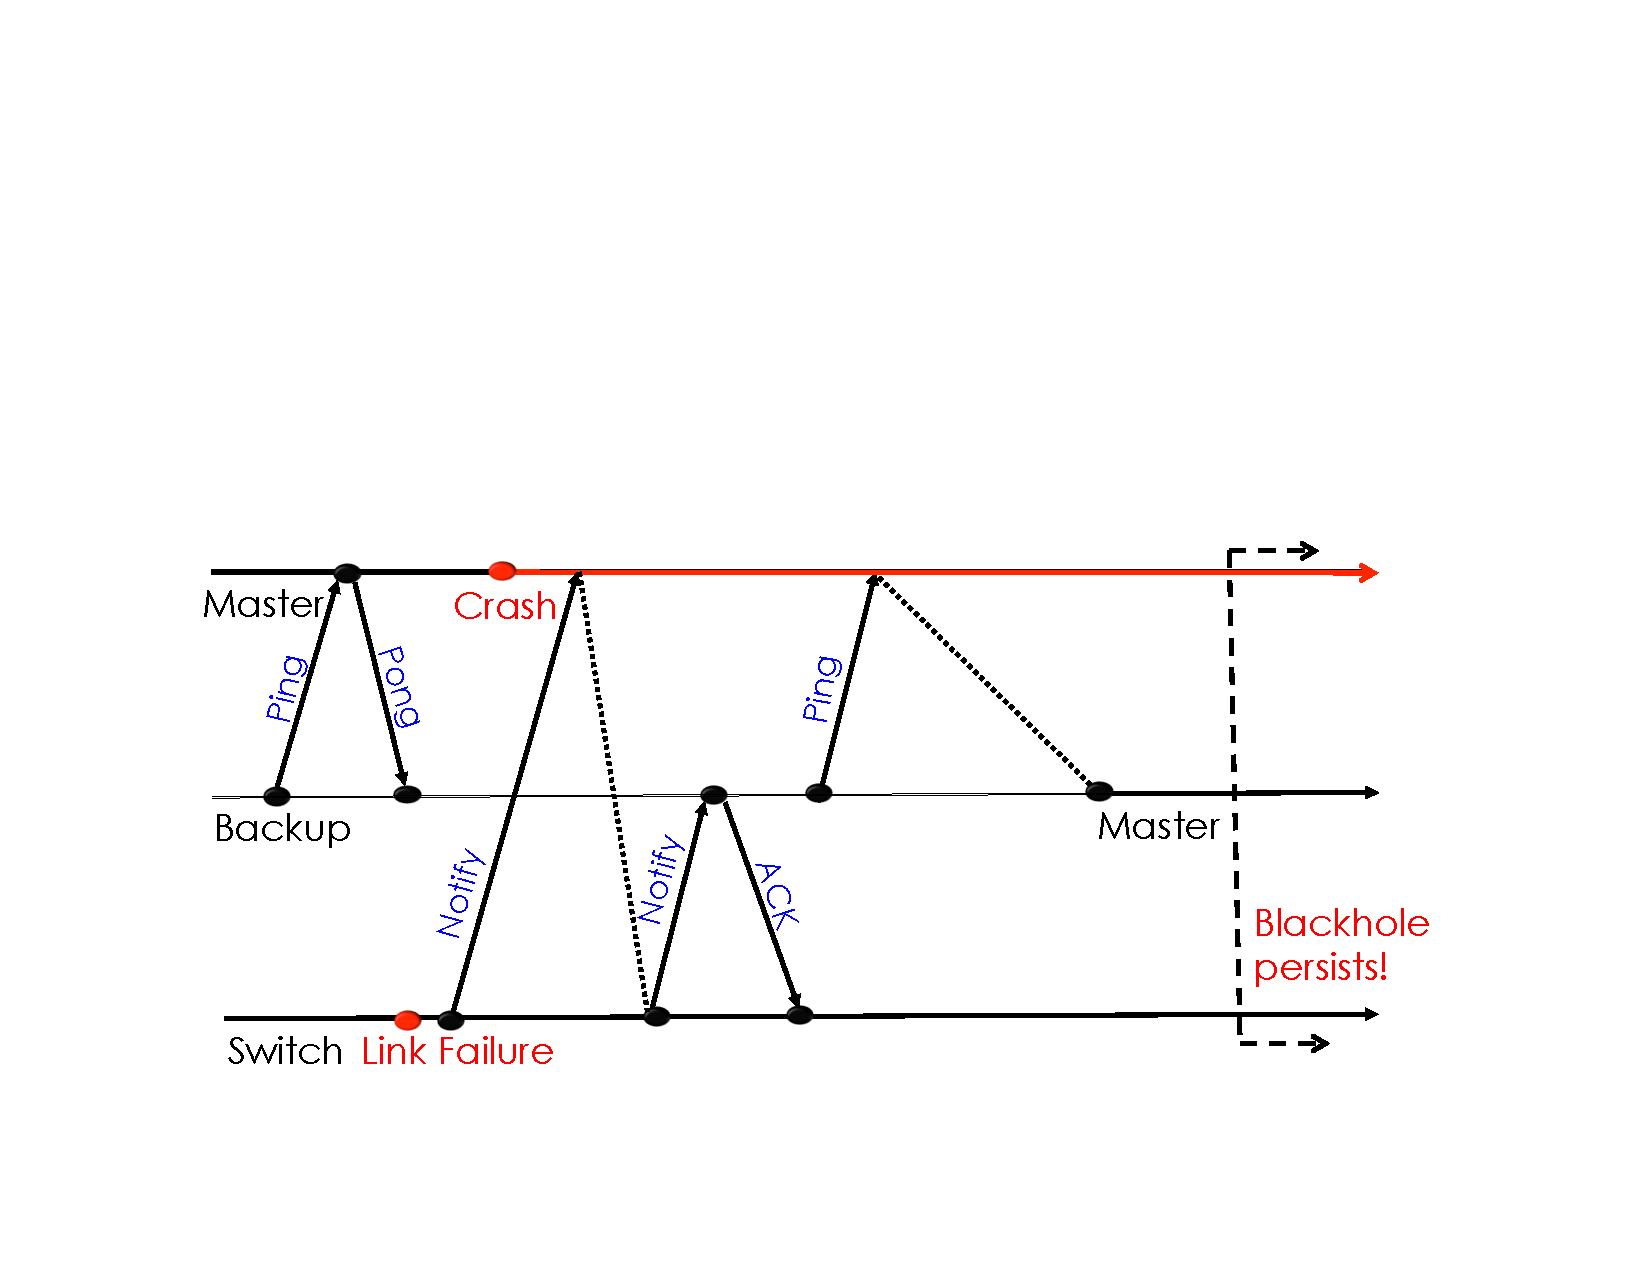
\includegraphics[width=3.25in]{../diagrams/case_study/example_bug.pdf}
  \caption[]{\label{fig:example} Floodlight failover bug. External inputs
             are depicted as red dots, internal events are depicted as black
             dots, and the dotted message line depicts a timeout.}
\end{figure}

The failover logic in Floodlight is incorrect, leading to the
following race condition\footnote{Note that this issue was
originally documented by the developers of Floodlight~\cite{floodlight_bug}.} depicted in
Figure~\ref{fig:example}:
a link fails (E1), and the switch attempts to notify the controllers (E2,E4) shortly after the master
controller has died (E3), but before a new master has been selected (E6). In this case, all live controllers are in
the backup role and will not take responsibility for updating the switch
flow table (E5). At some point, a backup notices the master failure and
elevates itself to the master role (E6). The new master will proceed to manage
the switch, but without ever clearing the routing entries for
the failed link, resulting in a persistent blackhole. In this example, the MCS
is the conjunction of the two external inputs (E1,E3).
}

\subsection{Searching for Subsequences}
\label{subsec:delta_debugging}

Checking random subsequences of $E_L$ would be one viable but inefficient
approach to achieving our first task. We do better by leveraging
%divide-and-conquer search technique from the software engineering community:
the delta debugging algorithm~\cite{Zeller:1999:YMP:318773.318946}, a
divide-and-conquer algorithm for
isolating fault-inducing inputs. In our case, we use delta
debugging to iteratively select subsequences of $E_L$ and replay each
subsequence with some timing $T$. If the bug persists for a given subsequence, delta debugging ignores the
other inputs, and proceeds with the search for an MCS within this subsequence.
%In what follows, we use the term {\em delta debugging} to refer to our algorithm for finding relevant subsequences.
The delta debugging algorithm is shown in Figure~\ref{fig:ddmin}.
%(with `$test$' replaced by `$replay$').

The input subsequences chosen by delta debugging are not always
valid. Of the possible inputs sequences we generate (shown in
Table~\ref{tab:inputs}), it is not sensible to replay a recovery event without a
preceding failure event, nor to replay a host migration
event without modifying its starting position when a preceding host
migration event has been pruned. Our implementation of delta debugging
therefore prunes failure/recovery event pairs as a single unit, and updates initial host locations
whenever host migration events are pruned so that hosts do not magically appear at new
locations.\footnote{Handling invalid inputs is crucial for
ensuring that the delta debugging algorithm finds a minimal causal
subsequence. The algorithm we employ~\cite{Zeller:1999:YMP:318773.318946}
makes three
assumptions about inputs: monotonicity, unambiguity, and consistency.
An event trace that violates monotonicity may contain events that ``undo'' the
invariant violation triggered by the MCS, and may therefore exhibit slightly
inflated MCSes. An event trace that violates unambiguity may exhibit multiple MCSes; delta debugging
will return one of them. The most important assumption is consistency, which
requires that the test outcome can always be determined.
We guarantee neither monotonicity nor unambiguity, but we guarantee consistency by
ensuring that subsequences are always semantically valid by applying the two
heuristics described above. Zeller wrote a follow-on
paper~\cite{Zeller:2002:SIF:506201.506206} that removes the need for these
assumptions, but incurs an additional factor of $n$ in complexity in doing so.}
These two heuristics account for validity of all network
events shown in Table~\ref{tab:inputs}. We do not yet
support network policy changes as events, which have more complex semantic
dependencies.\footnote{If codifying the semantic dependencies of
policy changes turns out to be difficult, one could just employ the more
expensive version of delta debugging to account for
inconsistency~\cite{Zeller:2002:SIF:506201.506206}.}

\begin{figure*}[t]
\begin{boxedminipage}{\textwidth}
Input: $\cfail$ s.t. $\cfail$ is a trace and $\test(\cfail) = \DFAIL$. Output: $\dfail
= \ddmin(\cfail)$ s.t. $\dfail \subseteq
\cfail$, $\test(\dfail) = \DFAIL$, and~$\dfail$ is minimal.
\begin{align*}
\ddmin(\cfail) &= \ddmin_2(\cfail, \emptyset) \quad \text{where} \\
\ddmin_2(\dfail, R) &=
\begin{cases}
\dfail & \text{\hphantom{else }if $|\dfail| = 1$ (``base case'')} \\
\ddmin_2\bigl(\done, R\bigr) &
\text{else if $\test(\done \cup R) = \DFAIL$ (``in $\done$'')} \\
\ddmin_2\bigl(\dtwo, R\bigr) &
\text{else if $\test(\dtwo \cup R) = \DFAIL$ (``in $\dtwo$'')} \\
\ddmin_2\bigl(\done, \dtwo \cup R\bigr) \cup \ddmin_2\bigl(\dtwo, \done \cup
R\bigr) & \text{otherwise (``interference'')}
\end{cases}
\end{align*}
\begin{center}
where $\test(T)$ denotes the state of the system after executing the trace $T$,
$\DFAIL$ denotes a correctness violation, \\
$\done \subset \dfail$, $\dtwo \subset \dfail$, $\done \cup \dtwo = \dfail$, $\done \cap
\dtwo = \emptyset$, and $|\done| \approx |\dtwo| \approx |\dfail| / 2$
hold.
\end{center}
\end{boxedminipage}
\caption{\colin{Cut if we need space} Automated Delta Debugging Algorithm From~\cite{Zeller:1999:YMP:318773.318946}}
\label{fig:ddmin}
\end{figure*}

\eat{ % Original O(n^2) algorithm
\begin{figure*}[t]
\caption{Minimizing Delta Debugging Algorithm From~\cite{Zeller:2002:SIF:506201.506206}}
\begin{boxedminipage}{\textwidth}
Input: $\cfail$ s.t. $\cfail$ is a trace and $\test(\cfail) = \FAIL$. Output: $\dfail
= \ddmin(\cfail)$ s.t. $\dfail \subseteq
\cfail$, $\test(\dfail) = \FAIL$, and~$\dfail$ is 1-minimal.
\begin{align*}
\ddmin(\cfail) &= \ddmin_2(\cfail, 2) \quad \text{where} \\
\ddmin_2(\dfail, n) &= 
\begin{cases}
\ddmin_2(\Delta_i, 2) & \text{\hphantom{else }if $\exists i \in \{1, \dots, n\} \cdot \test(\Delta_i) = \FAIL$ (``reduce to subset'')} \\
\ddmin_2\bigl(\nabla_i, \max(n - 1, 2)\bigr) & 
\text{else if $\exists i \in \{1, \dots, n\} \cdot \test(\nabla_i) = \FAIL$ (``reduce to complement'')} \\
\ddmin_2\bigl(\dfail, \min(|\dfail|, 2n)\bigr) & \text{else if $n < |\dfail|$ (``increase granularity'')} \\
\dfail & \text{otherwise (``done'').}
\end{cases}
\end{align*}
where $\test(T)$ denotes the state of the system after executing the trace $T$,
$\FAIL$ denotes a correctness violation, \\
$\nabla_i = \dfail - \Delta_i$, $\dfail = \Delta_1 \cup \Delta_2 \cup \dots \cup \Delta_n$, all
$\Delta_i$ are pairwise disjoint sequences of inputs, and $\forall \Delta_i \cdot |\Delta_i| \approx |\dfail| / n$
holds.
\end{boxedminipage}
\label{fig:ddmin}
\end{figure*}
}

\subsection{Searching for Timings}
\label{subsec:algorithm}

Simply exploring subsequences of $E_L$ is insufficient for finding MCSes: the
timing of those subsequences in each invocation of $replay()$ is crucial for reliably
reproducing the
invariant violation. The most natural approach would be to maintain the original
timings between the remaining original inputs for each subsequence.
\eat{\ie~if we
define $t_i$ as the timestamp of the $i^{th}$ input from the original run and $t'_i$ as the
replay clock value when it injects that same input
(which may or may not be the $i$'th input in the subsequence), then we might
just set $t'_i = t_i$.
\eat{
\begin{align*}
t'_0 = t_0 \\
t'_i = t'_{i-1} + |t_{i} - t_{i-1}|
\end{align*}
}
}
Unfortunately, this approach does not work in practice because it can violate
causal dependencies from the original execution, due to changes in the behavior
of the control software induced by pruning inputs. %\eat{: when we replay only a
%subsequence of the original inputs, the reaction of the control software
%can change, such that it behaves differently or takes a different amount of
%time to respond to the remaining inputs events.
%In practice we have observed that simply maintaining relative timings can
%result in injecting the remaining inputs too early or late.}
To reliably reproduce the invariant violation
we need to inject an input event $e$ only after all other
events, including internal events triggered by the control software itself,
that precede it in the
happens-before~\cite{Lamport:1978:TCO:359545.359563}
relation ($\{i \mid i \rightarrow e\}$) from the original execution have
occurred~\cite{tel2000introduction}.

Internal events include
(a) message delivery events, either between controllers (\eg~database
synchronization messages) or
between controllers and switches (\eg~OpenFlow commands), and (b) state transitions
within controllers (\eg~a backup node deciding to become master).
We obtain visibility into (a) by having our
\tester~(to be described in \S\ref{sec:systems_challenges}) interpose on all message channels.
We optionally obtain visibility into (b) by instrumenting controller
software with a simple interposition layer (to be described in \S\ref{subsec:mitigating}).
With visibility into internal events and control over input events, the
\tester~records a totally-ordered trace by logging an event only after
all prior events are completed.

%\subsection{Preserving Causality}

Maintaining the happens-before relation from the original trace
(which reproduces the violation) throughout replay of subsequences of the
trace (which may or may not reproduce that
violation) involves three issues: coping with syntactic differences in internal
events across runs,
handling internal events from the original
execution that may not occur after pruning, and dealing with new internal events that were not
observed at all in the original execution.

\eat{
\colin{Somewhat redundant. Maybe wait until use cases.}
While the inputs and original internal events are given to us,
we become aware of new internal events throughout replay by
(i) monitoring
control message receipts between controllers and switches,
and (ii) interposing on the controllers' logging library and notifying the
replayer whenever the control software executes a log statement (which serve to mark relevant state
transitions). Note that to achieve truly deterministic
replay, these log statements would need to
be highly granular, capturing information such as thread scheduling decisions;
we show in \S\ref{subsec:case_studies}
however that pre-existing, course granular log statements are often sufficient to
successfully reproduce bugs.}

%\footnote{We discuss this problem further in
%\S\ref{subsec:domain_knowledge}.}
%Note that the developer must provide enough logging statements
%so that relevant internal state transitions are captured and visible to our
%tool.

\begin{table}[tb]
\centering
\footnotesize
\begin{tabular}{|l|l|}
\hline
Internal message & Masked values \\
\hline
\hline
OpenFlow messages & xac id, cookie, buffer id, stats \\
% port numbers?
\hline
packet\_out/in payload & all values except src, dst, data \\
\hline
Log statements & varargs parameters to printf \\
\hline
\end{tabular}
\caption{Internal messages and their masked values. %The masks serve to
%define equivalence classes.
}
\label{tab:fingerprints}
\vspace{-0.5cm}
\end{table}


{\bf Functional Equivalence. } Internal events may differ syntactically (\eg~sequence numbers
of control packets may all differ) when replaying a subsequence of the original log.
We observe that many internal events are {\em functionally
equivalent}, in the sense that they
have the same effect on the state of the system with respect to triggering the
invariant violation (despite syntactic differences). For example, \emph{flow\_mod}
messages may cause switches to make the same change to their forwarding behavior
even if the transaction ids differ.

We leverage this observation by defining
masks over semantically extraneous fields of
internal events.\footnote{One consequence
of applying masks is that bugs involving masked fields are outside the purview of
our approach.} These masks only need to be specified once, and can later be
applied programmatically to event traces.

We show the fields we mask in Table~\ref{tab:fingerprints}. We consider an
internal event $i'$ observed in the replay
equivalent (in the sense of inheriting all of its happens-before relations) to an internal
event $i$ from the original log if and only if all unmasked fields have the same value
and $i$ occurs between $i'$'s preceding and succeeding inputs in the
happens-before relation.

\begin{table}[tb]
\centering
\footnotesize
\begin{tabular}{|l|l|}
\hline
\textbf{Input Type} & \textbf{Implementation} \\
\hline
\hline
Switch failure/recovery & TCP teardown \\
\hline
Controller failure/recovery & \verb=SIGKILL= \\
\hline
Link failure/recovery & \verb=ofp_port_status= \\
\hline
Controller partition & \verb=iptables= \\
\hline
Dataplane packet injection & Network namespaces \\
\hline
Dataplane packet drop & Dataplane interposition \\
\hline
Dataplane packet delay & Dataplane interposition \\
\hline
Host migration & \verb=ofp_port_status= \\
\hline
Control message delay & Controlplane interposition \\
\hline
Non-deterministic TCAMs & Modified switches \\
\hline
\end{tabular}
\caption{Input types currently supported by \projectname}
\label{tab:inputs}
\end{table}

\eat{
\begin{figure}[t]
    %\hspace{-10pt}
    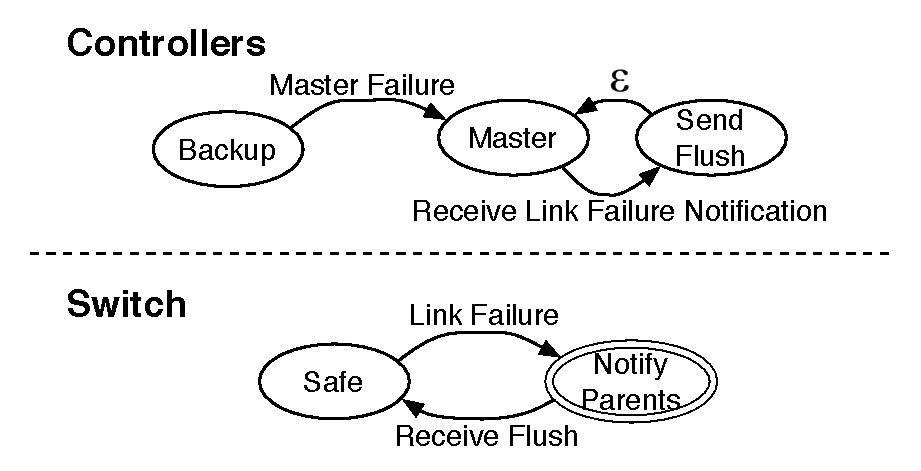
\includegraphics[width=3.25in]{../diagrams/state_machines/controller_switch.pdf}
    \caption[]{\label{fig:state_machines} Simplified state machines for the switch and
    controllers in the example Floodlight bug. Double outlined states
    represent presence of the blackhole.}
\end{figure}
}

{\bf Handling Absent Internal Events. } Some internal events from the original
log which causally ``happen before'' some external input
may be absent when replaying a subsequence of that log.
For instance, if we prune a link failure event, then
the corresponding link failure notification will never arise as an internal event.
\eat{
The control software's state machine (which we do not assume to know) determines whether
internal events cease to appear. Consider the simplified state machines for the switch and
controllers from the Floodlight case shown in
Figure~\ref{fig:state_machines}. If we prune the link failure input, the
master will never receive a link failure notification and
transition to and from \emph{Send Flush}.}

We handle this by attempting to infer the presence of internal
events before we replay each subsequence. Our algorithm (called {\sc Peek()}) for inferring the
presence of internal events is depicted in
Figure~\ref{fig:peek}. The algorithm injects each input, takes a
snapshot\footnote{We discuss the implementation details of snapshotting
in~\ref{subsec:snapshotting}.} of
the network and the control software's state, allows the system to proceed up
until the following input (plus a small time $\epsilon$), records the observed
events, and matches the
recorded events with the functionally equivalent internal events observed in
the original trace. With these inferred causal dependencies, we then replay
the subsequence, this time waiting to inject each input until each of its
(functionally equivalent) predecessors have occurred.\footnote{In the
case that, due
to non-determinism, an internal event occurs during {\sc Peek()} but does not occur
during replay, we time out on internal events after $\epsilon$ seconds of
their expected occurrence.}

\eat{ % Old version without peek()
We handle this possibility by waiting for each expected internal event
for a certain time \textepsilon. If the internal event does not occur within
this time, we assume that it is absent and proceed. If, however, we find
during the \textepsilon~time units we were waiting that another internal that
happens \emph{after} our next input occurs, we know that we have waited too
long and violated causality. In this case we need to restart the replay
process, this time knowing which internal events in the current
input interval are and are not going to occur before injecting the next input.
We show our overall event scheduling algorithm
in Figure~\ref{fig:replay}.
}

\eat{ % Somewhat redundant with peek()
\begin{figure}
  \begin{pseudocode}[framebox]{CausalInference}{events}
    \PROCEDURE{Replay}{subsequence}
    subsequence \GETS \CALL{Peek}{subsequence} \\
    \FOR e\textsubscript{i}\ in\ subsequence \\
      \BEGIN
      \IF e\textsubscript{i}\ is\ an\ internal\ event \\
      \AND e\textsubscript{i}\ is\ not\ marked\ absent:
      \THEN
        \BEGIN
          \Delta \GETS |e\textsubscript{i}.time - e\textsubscript{i-1}.time| + \epsilon \\
          wait\ up\ to\ \Delta\ seconds\ for\ e\textsubscript{i} \\
          \IF e\textsubscript{i}\ did\ not\ occur:
          \THEN mark\ e\textsubscript{i}\ as\ absent
        \END
      \ELSEIF e\textsubscript{i}\ is\ an\ input:
      \THEN
        \BEGIN
          \IF a\ successor\ of\ e\textsubscript{i}\ occurred: \\
          \INLINECOMMENT{waited too long}
          \THEN
            \RETURN{\CALL{Replay}{subsequence}}
          \ELSE
            inject\ e\textsubscript{i}
          \END
        \END
    \ENDPROCEDURE
  \end{pseudocode}
  \caption{{\tt Replay} is responsible for replaying subsequences of events
  chosen by delta debugging and determining
  if the bug reappears. \colin{Fix framebox width.}}
    \label{fig:replay}
\end{figure}
}

\begin{figure}
  \begin{pseudocode}[framebox]{Peek}{events}
    \footnotesize
    \PROCEDURE{Peek}{input\ subsequence}
    inferred \GETS [\ ] \\
    \FOR e\textsubscript{i}\ in\ subsequence \\
    \BEGIN
      snapshot\ system \\
      inject\ e\textsubscript{i} \\
      \Delta \GETS |e\textsubscript{i}.time - e\textsubscript{i-1}.time| + \epsilon \\
      record\ events\ for\ \Delta\ seconds \\
      matched \GETS original\ events\ \&\ recorded\ events \\
      inferred << e\textsubscript{i} << matched \\
      restore\ snapshot \\
    \END \\
    \RETURN{inferred}
    \ENDPROCEDURE
  \end{pseudocode}
  \caption{{\sc Peek} is responsible for determining which internal events
  from the original sequence are going to occur for a given subsequence.
  \label{fig:peek}}
\end{figure}

{\bf Handling New Internal Events.} The last possible change induced by pruning is the occurrence of new
internal events that were not observed in the original log.
New events present multiple possibilities for where
we should inject the next input. Consider the following case:
if $i_2$ and $i_3$ are internal events observed
during replay that are both in the same equivalence class as a single event $i_1$ from the
original run, we could inject the next input after $i_2$ or after $i_3$.

% TODO: figure this figure out
%\begin{wrapfigure}{c}{1.3\linewidth}
%  \centering
%  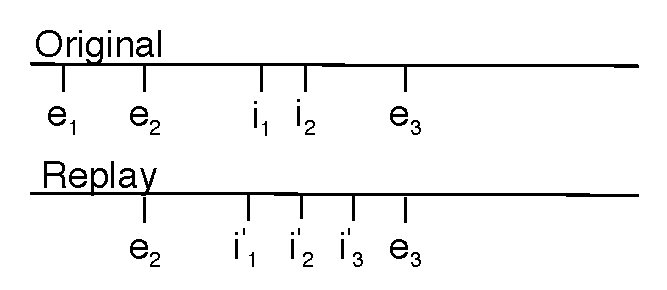
\includegraphics[width=\linewidth,height=0.8in]{../diagrams/state_machines/event_sequence.pdf}
%\end{wrapfigure}

In the general case it is always possible to construct two state machines that lead
to differing outcomes: one that only leads to the invariant violation when
we inject the next input
\emph{before} a new internal event, and another only when we inject \emph{after} a new internal
event. In other words, to be guaranteed to traverse any existing suffix that leads
to the invariant violation, we must recursively branch, trying both
possibilities for every new internal event. This implies an exponential number of
possibilities to be explored in the worst case.

Exponential search over these possibilities is not a practical option. Our heuristic when waiting for expected internal
events is to proceed normally if there are new internal events,
always injecting the next input when its last expected predecessor
either occurs or times out. This ensures that we always find suffixes that
contain a subset of the (equivalent) original internal events, but leaves open the
possibility of finding divergent suffixes that lead to the invariant
violation.
%This is reasonable because not even branching on new
%internal events is guaranteed to find the globally shortest fault-inducing input
%sequence:
%there may be other unknown
%paths through the state machine leading to the invariant violation that are
%completely disjoint from the original execution.

\eat{
Luckily, crucially ambiguous new internal events are not problematic for the
control software we evaluated, as we show in \S\ref{sec:casestudies}.
We conjecture that ambiguous new internal events are
rare because SDN software is a control plane system,
and is designed to quiesce quickly (\ie~take a small number of internal
transitions after any input event, and stop at highly connected vertices).
Concretely, SDN programs are often structured as (mostly independent) event
handlers, meaning that pruning input events simply triggers a subset of the original
event handlers.
\eat{
As an illustration, consider the state machines
in Figure~\ref{fig:state_machines}:
the controllers quickly converge to a single state (either ``Master'' or
``Backup''), as do the switches (``Safe'').
}
}

\subsection{Complexity}
\label{subsec:complexity}

The delta debugging algorithm terminates after $\Omega(\log n)$
invocations of $replay$ in the best case, and $O(n)$ in the worst case, where $n$ is the number of inputs in the original
trace~\cite{Zeller:1999:YMP:318773.318946}.
Each invocation of $replay$ takes $O(n)$ time
(one iteration for {\sc Peek()} and one iteration for the replay itself),
for an overall runtime of $\Omega(n \log n)$ best case and $O(n^2)$ worst case replayed inputs.
The runtime can be decreased by parallelizing delta debugging:
speculatively replaying subsequences in parallel, and joining the results.
Storing periodic checkpoints of the system state throughout testing can also reduce runtime, as it
allows us to replay starting from a recent checkpoint rather than the beginning of the
trace.% \barath{But doesn't this approach break due to non-determinism?  Sometimes we want
%a replay run to be different from a previous replay run...} 

\eat{
SDN platform developers can reduce the probability that the replay algorithm
will need to back up by placing causal annotations on internal
events~\cite{fonseca2007x}: with explicit causal information, the replay
algorithm can know
\apriori~whether certain internal events are dependent on pruned inputs.
}

\colin{Describe Andrew's input type pruning optimization and measurements. "We
make another optimization.."}

% In the next section we describe some of the practical challenges we have overcome to realize our approach.

% \colin{Cut this section?}
% In our initial experiments we have found that applying delta debugging to explore
% subsequences of $E_L$ and striving to maintain a single timing $T$ that maintains
% causal dependencies reliably finds small MCSes.


\vspace{-0.15in}
\section{INITIAL RESULTS}
\vspace{-0.1in}
\label{sec:init_results}
We have applied \simulator~to three open source SDN control platforms:
POX, NOX, and Floodlight. Over a span
of roughly five days of
investigation we found a total of five bugs. \Simulator~reduced the
size of the input trace to 37\% of its original size in
the worst case and 2\% of its original size in the best case.
We show the overall results of our case studies
in Table~\ref{tab:case_studies}.

\begin{table*}
\centering
\begin{tabular}{l|l|l|l|l}
Bug Name & Topology & Runtime & Total Inputs & MCS Size \\
\hline
POX list removal & 2 switch mesh & 141.0s & 76 (69) & 2 (2) \\
% Original: config/eugene_epsilon_replay.py
% MCS: config/eugene_epsilon_mcs.py
POX in-flight blackhole & 2 switch mesh & 2855.5s & 68 (26) & 25 (11) \\
% Original: 7ba95ed82ca4e32f12ab511d9c4301dbac2c59d5
% MCS: 399cf861db87a65e600283d9ae7760400c4676e2
POX migration blackhole & 4 switch mesh & 1796.0s & 117 (29) & 3 (2) \\
% fuzz_pox_4mesh_blackhole on pox_blackhole branch
NOX discovery loop & 4 switch mesh & 20237.6s & 358 (150) & 58 (18) \\
% Original: ce547fc1df3bde279b6f3dd589c909663e295f1e
% MCS: 5f49e791b0c1a611454cf0930f54aa609dd635d3
Floodlight loop & 3 switch mesh & analysis pending & analysis pending & analysis pending\\
% Andi
\end{tabular}
\caption{Overview of bugs found and MCS results. Totals shown in parentheses
exlude dataplane permit events.}
\label{tab:case_studies}
\end{table*}

We briefly describe one bug in POX's routing module to illustrate the value of minimal causal sets.
We noticed that our tool reported a persistent blackhole between two hosts A
and B while POX was bootstrapping its
discovery of link and host locations. There were 68 inputs in the initial trace, and \simulator~returned a 25 input
MCS. With the MCS in hand we took out paper and pencil to decipher what had
transpired.

We found that the crucial triggering events were two
{\em in-flight} packets (set in motion by prior traffic injection events),
concurrent with POX's discovery of a switch-switch link.
More specifically, we saw that directly after POX discovered the link connecting the two
switches, the first in-flight packet from host A arrived at
B's attached switch without a prior PacketIn from A's attached switch.
This was POX's first mistake: although it correctly realized that hosts cannot
be attached to the newly discovered switch-switch link, the code did not correctly handle in-flight packets
concurrent with the discovery of the link. As a result, it incorrectly learned A's location at
the switch-switch link.

The next event we observed was another in-flight packet arriving from B to
A. POX
proceeded to install a path for this new B$\rightarrow$A flow, but the
path itself contained a loop! The default behavior of
OpenFlow switches is to ignore route entries (with wildcarded
IN\_PORTs) that forward out the
same port the packets arrived on. This is where we started observing the blackhole:
now whenever B sent traffic to A, it would be dropped until
the faulty routing entry would eventually expire 30 seconds later.
Upon further examination, we found that the programmer had neglected to return out
of a nested conditional, causing a B$\rightarrow$A flow entry to be
installed at one too many switches.

These fine-grained race conditions would have been difficult to reproduce
in Mininet~\cite{handigol2012reproducible} or real hardware. With our
network simulator's capacity to arbitrarily delay messages, the bug was easily uncovered. And with
an MCS in hand, it was straightforward to identify the root cause from an
otherwise complicated trace.
We have sent the minimized, replayable bug trace to the lead
developer of POX, and await his response.


\vspace{-0.1in}
\renewcommand{\baselinestretch}{0.1}
\footnotesize{\bibliographystyle{abbrv}
\bibliography{bib}
}

%\input{appendix}

%\theendnotes

\end{document}
